\section{Technische Realisierung}
In diesem Kapitel gehen wir auf die technische Realisierung des Projektes ein. Im Abschnitt Domänenmodell werden zunächst die verwendeten Begriffe definiert. Anschließend wird auf die Architektur, das Datenmodell und die Authentifizierung der Benutzerrollen eingegangen. Abschließend beschreiben wir exemplarisch einen Methodenaufruf, mit dem die wichtigsten Komponenten des Systems vorgestellt werden.

\subsection{Domänenmodell}
\label{sec:Domaenenmodell}

\begin{description}
	\item [Roles]:
	\begin{itemize}
		\item Admin
			\begin{itemize}
				\item Verwaltet die Songs auf dem Server.
			\end{itemize}
		\item Party People
			\begin{itemize}
				\item Voten die Songs.
				\item Ist nach dem ersten Kontakt eindeutig identifizierbar (Party People ID).
			\end{itemize}
	\end{itemize}
	\item [Jukebox]: datenbankgestützte WildFly-Anwendung
	\begin{itemize}
		\item Verwaltung der Songs und Song-Informationen.
			\begin{itemize}
				\item Songs hinzufügen.
				\item Songs löschen.
				\item Song-Informationen bearbeiten.
			\end{itemize}
		\item Generierung und Verwaltung der Playlist.
	\end{itemize}
	\item [Song]:
		\begin{itemize}
			\item Hat Song-Information.
			\item Muss abspielbar sein.
				\begin{itemize}
					\item Pfad in Dateisystem
					\item Internetstream
					\item YouTube-Link
				\end{itemize}
		\end{itemize}
	\item [Song-Information]:
		\begin{itemize}
			\item Titel, Interpret, Genre, Album, Länge.
		\end{itemize}
	\item [Current Song]:
		\begin{itemize}
			\item Song der gerade gespielt wird.
			\item Wenn Current Song abgespielt ist, wird der erste Song aus der Playlist entfernt und zum Current Song.
		\end{itemize}
	\item [Playlist]:
		\begin{itemize}
			\item Absteigend sortierte Song Liste auf Basis des Votings.
			\item Playlist wird durch Playlist-Füll-Prozess generiert.
				\begin{itemize}
					\item Solange Größe Playlist nicht erreicht, wähle nächsten Song via Song-Selection.
				\end{itemize}
		\end{itemize}
	\item [Song-Selection]:
		\begin{itemize}
			\item Nächste Song wird auf Basis von DI, Party Time usw. ausgewählt.
			\item Aus globaler Song Liste der Jukebox.
		\end{itemize}
	\item [Voting]:
		\begin{itemize}
			\item Basiert auf Playlist.
			\item Erlaubt Party People Songs innerhalb der Playlist zu bewerten.
				\begin{itemize}
					\item Up-Vote
					\item Down-Vote
				\end{itemize}
			\item Vote v = Anzahl Up-Votes - Anzahl Down-Votes.
			\item Party People darf pro Song max. einmal voten.
		\end{itemize}
	\item [DI] :
		\begin{itemize}
			\item Beschreibt den Betrunkenheitsgrad der Party People.
			\item ganzzahliger Wert zw. 0 - 100.
		\end{itemize}
\end{description}



\subsection{Architektur}

\todo{Daniel}

- Systemübersicht / Komponentendiagramm
- Beans und deren Aufgaben

\begin{figure}[H]
	\centering
	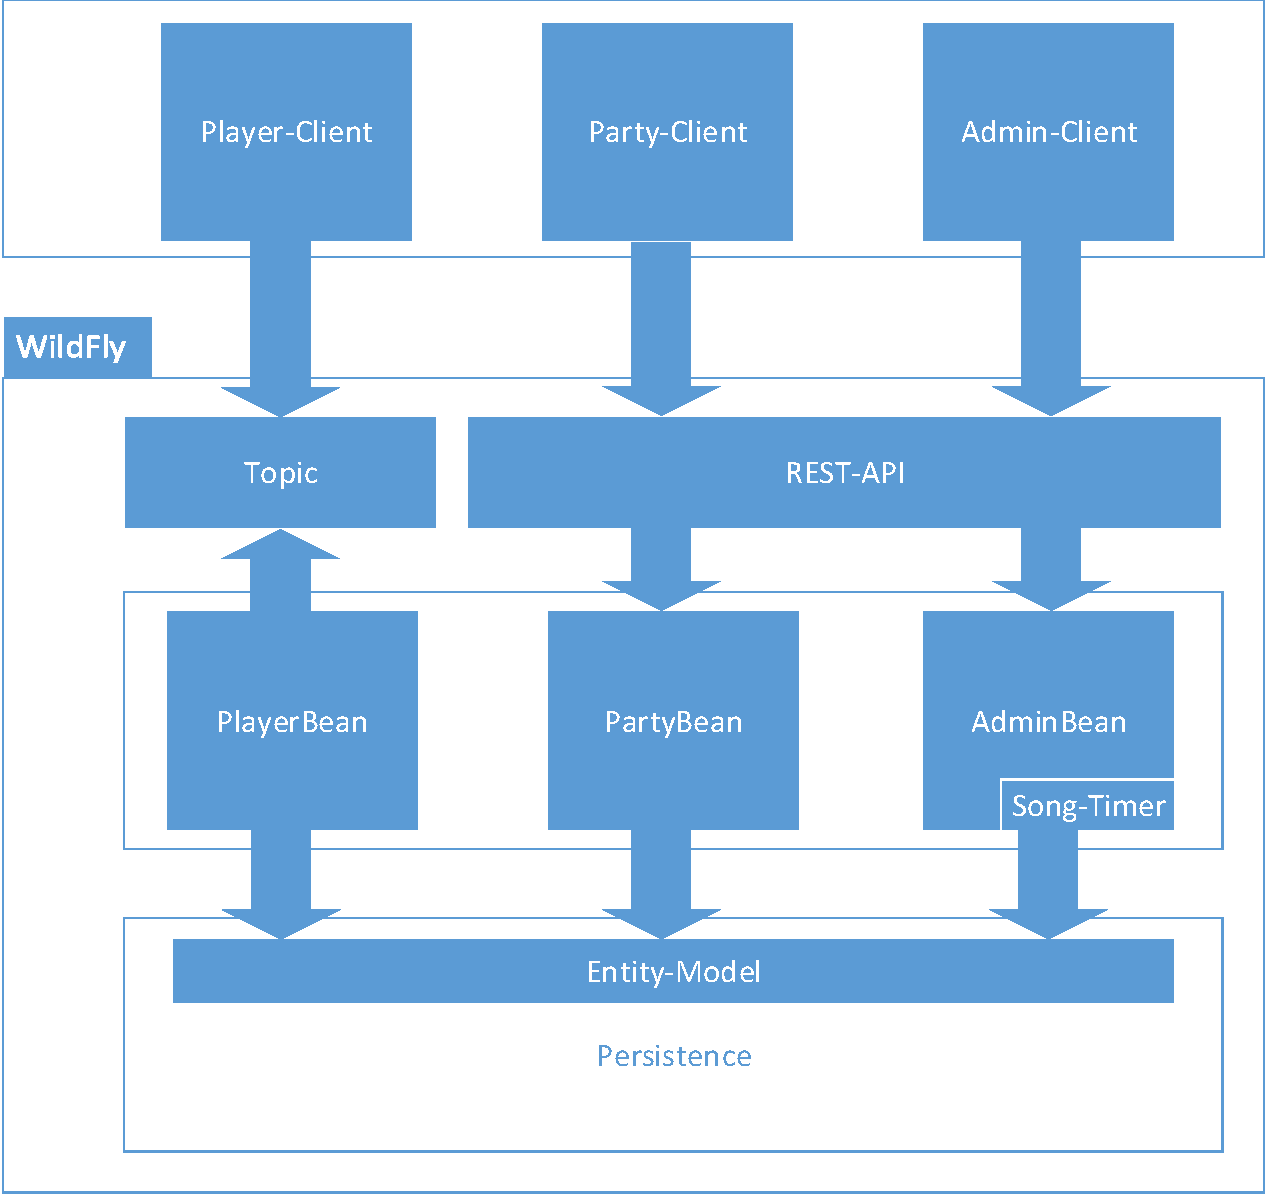
\includegraphics[width=1\linewidth]{Bilder/Komponentendiagramm}
	\caption{}
	\label{fig:Komponentendiagramm}
\end{figure}


\subsection{Datenmodell}

In diesem Abschnitt wird das Datenmodell beschrieben. Dieses besteht aus Entitäten für die Objekte aus dem \nameref{sec:Domaenenmodell}, die persistiert werden sollen. Benutzer- und Rollendaten werden im Abschnitt \ref{sec:Benutzerrollen} beschrieben.

\begin{figure}[htb]
\centering
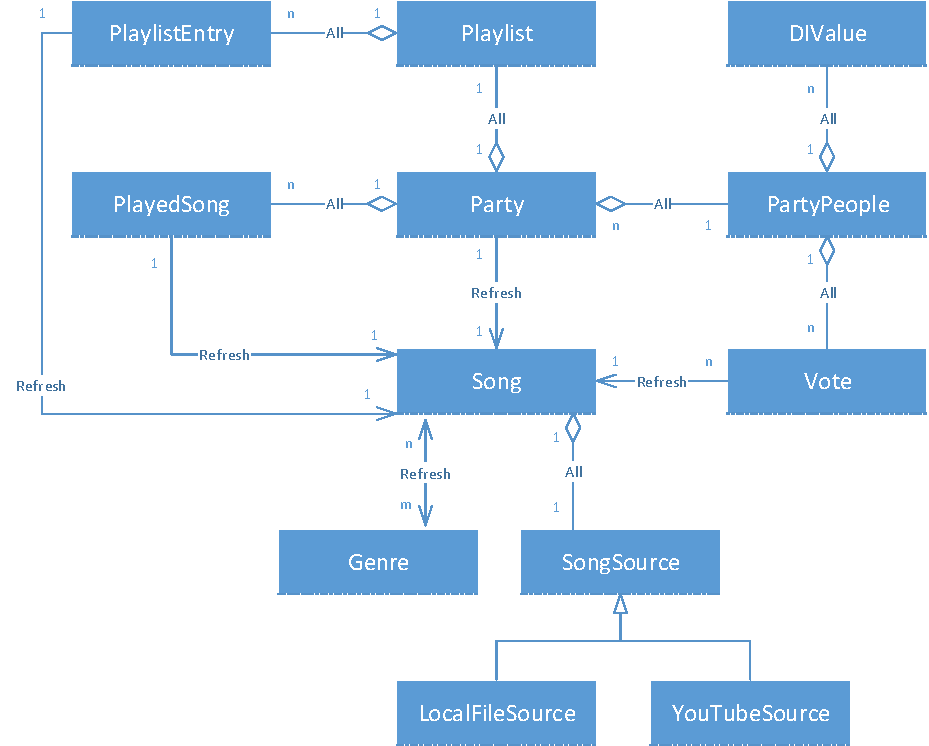
\includegraphics[width=1\linewidth]{Bilder/Datenmodell}
\caption{Datenmodell mit Beziehungen und Cascading zwischen Entitäten}
\label{fig:Datenmodell}
\end{figure}

Abbildung \ref{fig:Datenmodell} zeigt die Entitäten sowie deren Beziehungen untereinander. Neben der Kardinalität ist in dem Diagramm auch das Cascading-Verhalten dokumentiert. Wir haben zwei unterschiedliche Arten verwendet:
\begin{description}
	\item[Refresh] Eine Entität kennt eine andere Entität. Änderungen oder Löschoperationen werden nicht an die verknüpfte Entität weitergeleitet (Abhängigkeit).
	\item[All] Eine Entität besitzt eine andere Entität. 
	Änderungen oder Löschoperationen werden an die 
	verknüpfte Entität weitergeleitet (Aggregation).
\end{description}


\subsection{Benutzerrollen}
\label{sec:Benutzerrollen}
Die Authentifizierung und Autorisierung von Benutzer erfolgt über das Sicherheitskonzept im WildFly. Dazu werden Benutzerrollen für die unterschiedlichen Anwender definiert. Der Zugriff auf Beans sowie die REST-Services wird über diese Rollen geregelt. 

\subsubsection{Konzept}
Es gibt drei Benutzerrollen: Admin, Player und PartyPeople.
\begin{description}
	\item[Admin]: Ein Administrator hat Zugriff auf das Admin-Bean und den Admin-Service, um Songs und Partys zu verwalten.
	\item[Player]: Ein Player hat Zugriff auf das DJ-Topic, um Nachrichten zum Abspielen von Songs zu empfangen.
	\item[PartyPeople]: PartyPeople haben als Gäste der Party Zugriff auf das Party-Bean und den Party-Service.
\end{description}

\subsubsection{Umsetzung}
Die Benutzer- und Rollendaten werden in der Datenbank gespeichert. Dazu wurden die zwei Entitäten \texttt{Principal} und \texttt{Role} angelegt. In der Datenbank wird zur Zuordnung zwischen Benutzern und Rollen eine zusätzliche Verknüpfungstabelle angelegt. Die Tabellen werden in Abbildung \ref{fig:BenutzerRollen} dargestellt.

\begin{figure}[tbh]
\centering
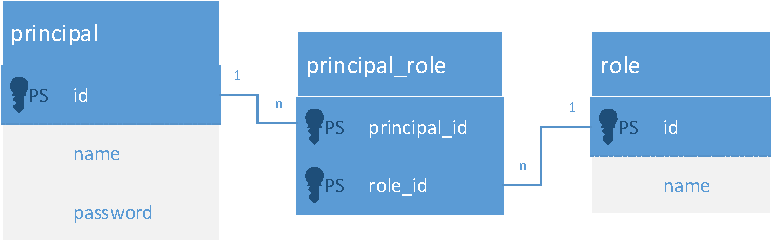
\includegraphics[width=1.0\linewidth]{Bilder/BenutzerRollen}
\caption{Tabellen für die Benutzerverwaltung}
\label{fig:BenutzerRollen}
\end{figure}

Im Standard verwendet WildFly die lokalen Benutzerdaten in den *.properties-Dateien. Um das Verhalten zu ändern, muss ein neues Login-Modul in der standalone.xml angelegt werden. In dieses Datenbank-Login-Modul die Datenquelle zusammen mit den SQL-Abfragen zur Bestimmung von Passwörtern und Rollen definiert werden. Aktuell werden die Passwörter im Klartext gespeichert. Für den produktiven Einsatz sollte hier auf ein aktuelles Hash-Verfahren wie SHA-2 umgestellt werden.

Um denselben Authentifizierungsmechanismus für Remote-Verbindungen und HTTP-Anfragen gegen den REST-Service zu nutzen, haben wie eine eigene Security-Realm sowie -Domain definiert. Zusätzlich war die Einstellung für Passwort-Stacking wichtig, da sonst entweder nur die Anmeldung über die REST-Schnittstelle oder über Remote möglich war. Die Zuordnung der Security-Domain zu den Beans und Services erfolgt über Annotationen an den entsprechenden Java-Klassen. 

\subsubsection{Probleme}
Die Authentifizierung war das größte Problem im gesamten Projekt, das entsprechend auch mit dem höchsten Arbeitsaufwand verbunden. Selbst nach stundenlanger Recherche konnten einige Probleme aufgrund der eher mangelhaften Dokumentation und der wenig hilfreichen Fehlermeldungen nicht oder nur teilweise gelöst werden.

Besonders auffällig war, dass die einzelnen Features wie Remote-Authentifizierung einfach einzurichten waren. Sollte dieselbe Authentifizierung auch für REST-Service genutzt werden, mussten aufwendige und nicht dokumentierte Anpassungen an der WildFly-Konfiguration vorgenommen werden. Als gegen Ende des Projekts auch das Messaging authentifiziert werden sollte, konnten wir keine Lösung finden, mit der alle drei Schnittstellen korrekt arbeiteten. Aktuell funktioniert die Authentifizierung für Remote- und HTTP-Verbindungen. 


\subsection{Exemplarische Darstellung}
\todo{Daniel}
- Beschreibung eines Funktionsaufrufes z.B. start Party durch alle "`Schichten"' des Systems

\begin{figure}[tbh]
\centering
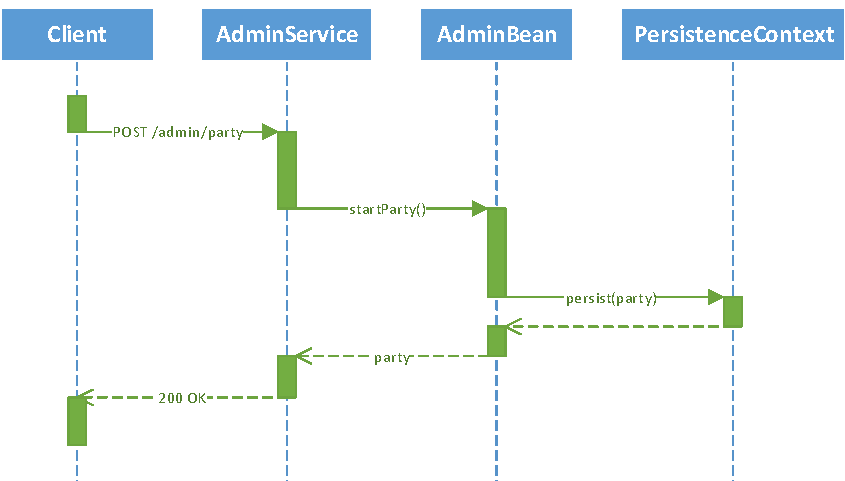
\includegraphics[width=1.0\linewidth]{Bilder/AufrufSequenz}
\caption{Sequenzdiagramm für den Start einer Party}
\label{fig:AufrufSequenz}
\end{figure}





